\documentclass[12pt]{article}
\usepackage[margin=1in]{geometry}
\usepackage{amsmath,amssymb}
\usepackage{graphicx}
\usepackage{booktabs}
\usepackage{array}
\usepackage[superscript]{cite}
\usepackage[hidelinks]{hyperref}
\makeatletter
\renewcommand{\@biblabel}[1]{#1.}
\makeatother
\setlength{\parskip}{4pt plus 1pt}
\title{Fundamental Information for Low-Turnover Equity ML}
\date{October 2026}

\begin{document}
\maketitle
\section*{Abstract}
\textbf{Background/Objective. }Most stock-prediction research targets price moves a few days ahead and evaluates models on prediction metrics, leaving open whether accuracy gains survive turnover and transaction costs as portfolios. This study asks whether slow-moving fundamental data, traded by a long-memory model as a low-turnover strategy, beats technical signals. \textbf{Methods. }A Mamba-inspired selective state space (MISS) model was trained on point-in-time SEC fundamental features (profitability, growth, valuation, balance-sheet strength) to predict 63-day sector-neutral forward returns for S\&P 500 stocks. LSTM, StockMixer, and graph neural network baselines, plus matched 63-day and 5-day technical regimes under identical rules. Walk-forward retraining covered test years 2021--2025; scores were traded as a sector-demeaned top-10/bottom-10 long-short book at 15 bps one-way cost and scored on return, Sharpe ratio, turnover, cost sensitivity, a block bootstrap, and the Deflated Sharpe Ratio. \textbf{Results. }The fundamental strategy returned 17.53\% per year at Sharpe 1.104 with about 32 trade events per year, against $-6.84\%$ ($-0.299$) for matched long-horizon technicals and $-4.48\%$ ($-0.276$, 605 events) for 5-day technicals. The block bootstrap gave $\Pr(\mathrm{Sharpe~gap} > 0) = 0.988$; the fundamental strategy was the only one of twelve configurations with Deflated Sharpe near 1.0, and MISS led every architecture on fundamentals. \textbf{Conclusions. }Fundamental information pays when the horizon matches how slowly fundamentals change, and selective state-space memory suits sparse fundamental data. The edge is regime- and architecture-dependent, and the trained technical scores carried no out-of-sample signal. \textbf{Keywords: }financial machine learning; fundamental data; state space models; Mamba; long-horizon trading; walk-forward validation; transaction costs.

\section{Introduction}
Stock price prediction is a core problem in financial machine learning, and neural networks are widely used for it because they fit nonlinear market structure\cite{fischer2018,gkx2020}. Prices move on fundamentals, technicals, and sentiment: earnings and balance sheets set value, order flow and volatility move prices in the short run, and news shocks move investor psychology. The Sharpe ratio is the natural score for a strategy, since it prices the volatility a return costs. Financial data is noisy, nonstationary, and short---about 250 trading days a year per stock---yet nonlinear models have found useful signals in large panels\cite{fischer2018,gkx2020}, and algorithmic trading already relies on such models\cite{lopez2018}.

Most published models aim a few days out and are scored on prediction metrics, which says little about whether a small accuracy gain survives turnover and transaction costs once it becomes a portfolio\cite{fischer2018,demiguel2020}. A model can also have lower prediction error and still lose money if it trades too much or fails in volatile stretches, and testing many variants can fake significance\cite{harvey2016}. Research needs strategies evaluated as portfolios, not just predictions.

This study tests a different combination: slow-moving fundamental data, a Mamba selective state space model whose input-dependent memory keeps important observations for months while letting noise fade\cite{gu2023}, and a sector-neutral portfolio designed to trade rarely. If the data's frequency, the model's memory, and the portfolio's trading frequency are matched, the result should be a more practical investment framework than a fancier short-term model.

The objectives are (1) to test whether long-horizon fundamental signals beat matched long-horizon and short-horizon technical signals as portfolios; (2) to compare MISS against LSTM, StockMixer, and GNN architectures under identical rules; and (3) to verify robustness to transaction costs, sampling variation, and multiple testing.

The study covers S\&P 500 stocks over out-of-sample years 2021--2025. Point-in-time fundamental coverage is incomplete (161--201 scored names per year versus 441--474 for technicals), five years cannot cover every market regime, and sector neutrality removes industry bets but not factor exposures.

The guiding idea is horizon matching: a feature's value depends on the horizon at which it is evaluated, so slow fundamentals should predict quarterly-scale returns, and the model's memory should run on the same slow clock\cite{shiller1981}.

Models are retrained yearly on expanding windows, scored daily, and traded as a concentrated long-short book; performance is reported as five-year means with bootstrap, sign-test, cost-sensitivity, and Deflated Sharpe diagnostics\cite{bailey2014}.

\section{Methods}
Walk-forward design. For each test year 2021--2025, the model trains on an expanding window ending two years prior, validates on the intervening year (checkpoints picked by validation RankIC), and tests on the target year, retrained at each annual boundary using only information available at that point.

S\&P 500 constituents. The fundamental regime scores 161--201 names per year, limited by point-in-time SEC filing coverage; the technical regimes score 441--474 names per year.

Daily open-high-low-close-volume data come from Yahoo Finance\cite{yahoo2026}. Fundamental accounting features (return on assets, operating margin, revenue and earnings growth, earnings and free-cash-flow yield, leverage, liquidity, accruals) are built from SEC EDGAR filings\cite{sec2025} and enter only after each filing's acceptance date, never backfilled. Technical features (multi-period returns, realized volatility, moving-average distance, RSI, MACD, ATR, volume surprise, price-volume trend) are computed from prices and volume. Features are winsorized on training-data thresholds and cross-sectionally standardized per date.

Four model types of about 0.2M parameters each see the same targets and portfolio rules: MISS (two selective state-space blocks plus a scoring head, trained with a Huber regression loss plus a pairwise ranking loss), LSTM\cite{hochreiter1997,rumelhart1986}, StockMixer (MLP mixing across indicators, time, and stocks)\cite{fan2024}, and GNN (message passing over sector and rolling return-correlation edges)\cite{feng2019,qian2024}. A Transformer was not used as a baseline because its quadratic attention cost is impractical for the 252-day input sequences here\cite{vaswani2017}.

The primary target is the 63-trading-day forward return minus the stock's sector mean return (sector-neutral stock selection); the technical benchmark uses a 5-day target. Model output is a daily score per stock. Portfolio outcomes are measured as annualized return, annualized Sharpe ratio ($\times\sqrt{252}$, risk-free zero), annual one-way turnover (traded notional divided by NAV), trade events per year (position entries plus exits), and maximum drawdown.

Each date, scores are demeaned within sector and ranked globally, following the concentrated long-short form of Fischer and Krauss\cite{fischer2018}: long the top 10 names, short the bottom 10, equal weight, 100\% long / 100\% short, approximately zero net market exposure. A held name is retained while its rank stays inside the top (bottom) 80, which lowers turnover. The 63-day books rebalance monthly and the 5-day book weekly; 15 basis points are charged per unit of one-way notional traded.

Metrics are computed per test year and averaged over the five years. Costs are swept from 0 to 50 basis points one-way. A 10,000-resample moving-block bootstrap (21-day blocks) estimates the distribution of the Sharpe difference between the fundamental and short-horizon technical strategies. Year-level one-sided exact sign tests compare yearly wins. The Deflated Sharpe Ratio\cite{bailey2014} adjusts the best Sharpe for the twelve configurations tested.

No human participants, surveys, or personal data are involved. All inputs are public market data and regulatory filings; no informed consent or confidentiality procedures apply.

\section{Results}
Table 1 reports the five out-of-sample years for MISS. The fundamental strategy returns 17.53\% per year at Sharpe 1.104 with about 32 trade events per year. The matched 63-day technical strategy returns $-6.84\%$ (Sharpe $-0.299$) with 254 events; the 5-day technical strategy returns $-4.48\%$ (Sharpe $-0.276$) with 605 events. The fundamental edge over the 63-day technical book is 24.37 percentage points of return and 1.403 of Sharpe; over the 5-day book, 22.01 points and 1.380. The edge is uneven across years: 2021 is negative ($-1.9\%$) while 2025 ($+46.4\%$) and 2023 ($+18.2\%$) carry the mean, and the fundamental strategy beats the 5-day technical strategy in three of five years on both return and Sharpe. Figure 1 shows \$1 compounding to \$2.13 for the fundamental book while both technical books end below \$0.71.

\begin{table}[t]
\centering\footnotesize
\caption{Five-year out-of-sample results for the MISS architecture, net of 15 bps one-way costs. ``Events'' are portfolio trade/rebalance events per year.}
\begin{tabular}{l rrr rrr rrr rrr}
\toprule
& \multicolumn{3}{c}{2021} & \multicolumn{3}{c}{2022} & \multicolumn{3}{c}{2023} & \multicolumn{3}{c}{2024} \\
\cmidrule(lr){2-4}\cmidrule(lr){5-7}\cmidrule(lr){8-10}\cmidrule(lr){11-13}
Strategy & Ret. & SR & Ev. & Ret. & SR & Ev. & Ret. & SR & Ev. & Ret. & SR & Ev. \\
\midrule
Fund. 63d & $-1.9$ & $-0.07$ & 34 & 23.0 & 1.49 & 22 & 18.2 & 1.47 & 34 & 1.9 & 0.23 & 36 \\
Tech. 63d & $-24.2$ & $-1.53$ & 226 & $-3.5$ & $-0.00$ & 274 & 10.6 & 0.77 & 328 & $-15.1$ & $-0.73$ & 162 \\
Tech. 5d & 12.6 & 0.88 & 514 & $-14.3$ & $-0.80$ & 658 & $-31.8$ & $-2.35$ & 678 & 24.8 & 1.62 & 578 \\
\bottomrule
\end{tabular}

\medskip
\begin{tabular}{l rrr rrr}
\toprule
& \multicolumn{3}{c}{2025} & \multicolumn{3}{c}{Five-year mean} \\
\cmidrule(lr){2-4}\cmidrule(lr){5-7}
Strategy & Ret. & SR & Ev. & Ret. & SR & Ev. \\
\midrule
Fund. 63d & 46.4 & 2.41 & 34 & 17.53 & 1.104 & 32 \\
Tech. 63d & $-2.0$ & $-0.00$ & 278 & $-6.84$ & $-0.299$ & 254 \\
Tech. 5d & $-13.8$ & $-0.73$ & 598 & $-4.48$ & $-0.276$ & 605 \\
\bottomrule
\end{tabular}
\end{table}
\begin{figure}[t]
\centering
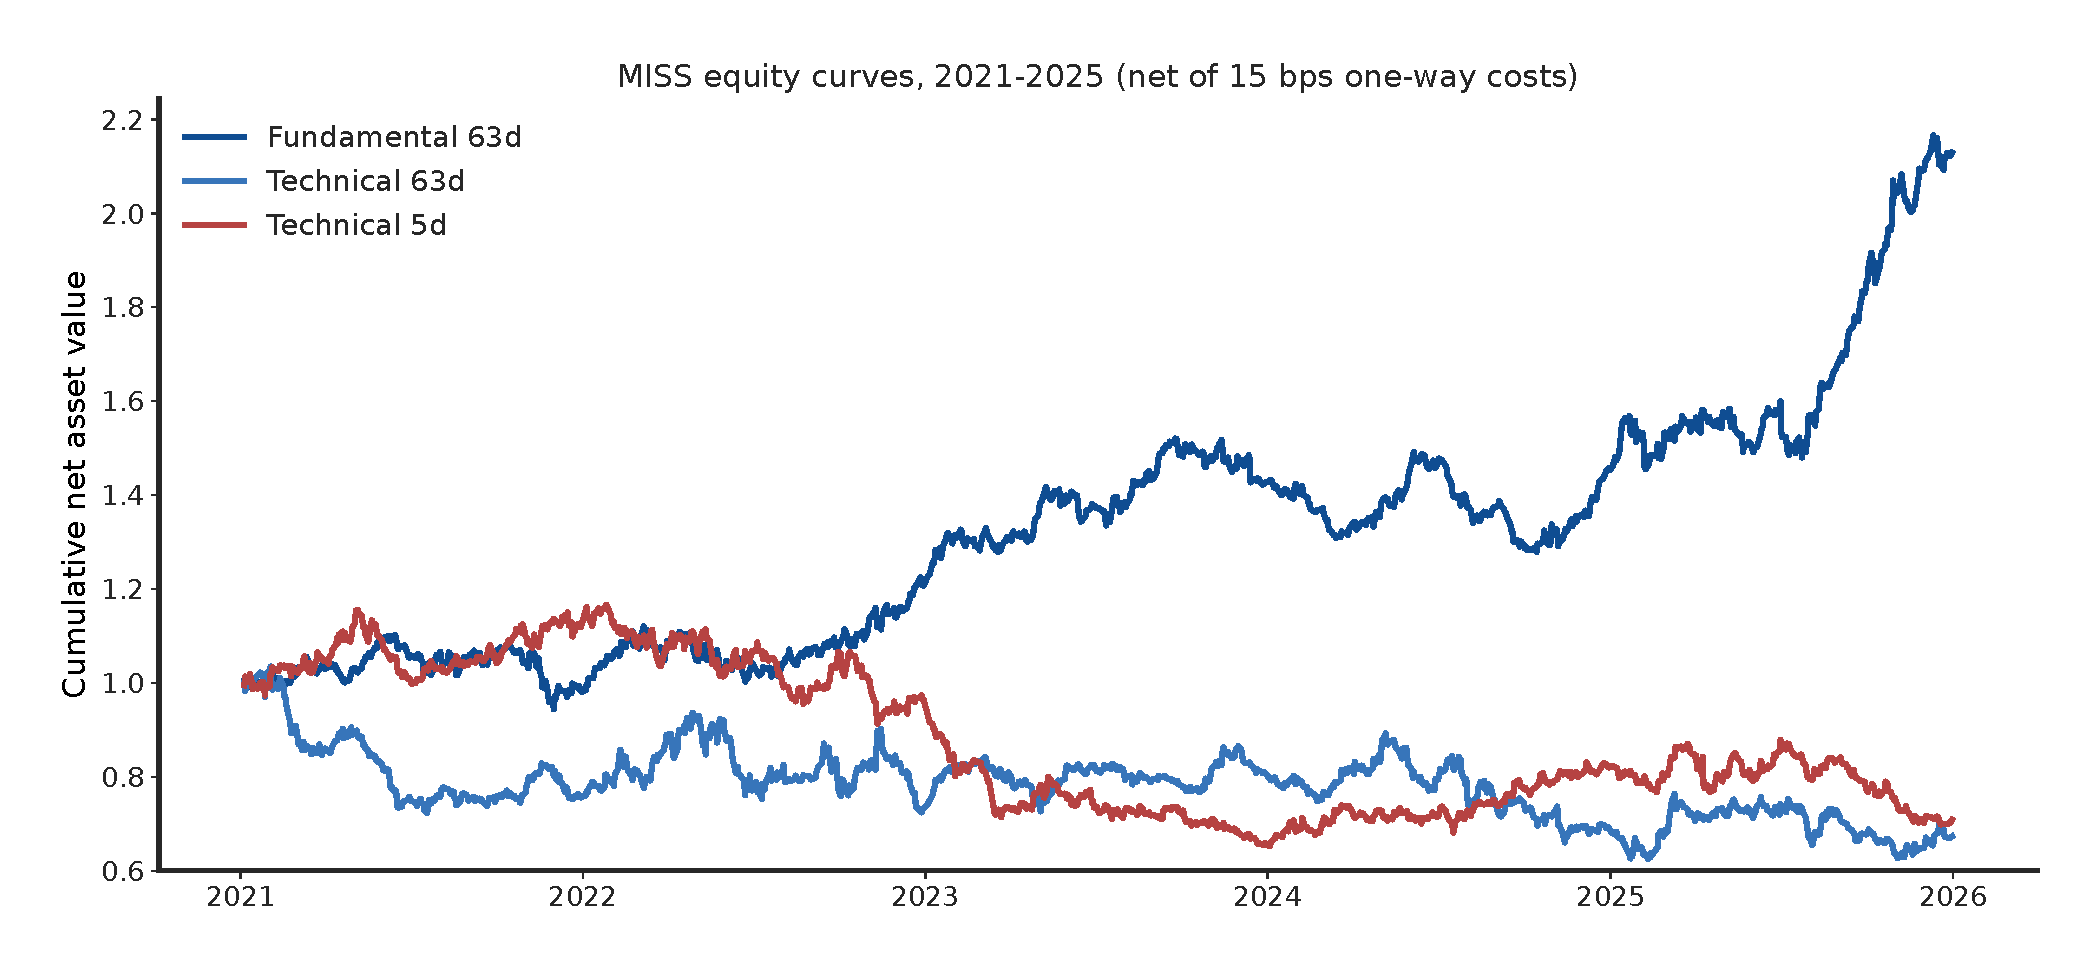
\includegraphics[width=0.92\textwidth]{figures/fig1_equity.pdf}
\caption{Cumulative net asset value of the three MISS information regimes, 2021--2025, net of 15 bps one-way costs. Fundamental 63d compounds \$1 to \$2.13; Technical 63d and 5d end at \$0.67 and \$0.71.}
\end{figure}
Table 2 compares architectures under identical rules. MISS leads the fundamental task (Sharpe 1.104), ahead of GNN (0.839), LSTM (0.665), and StockMixer ($-0.239$). On technical tasks nothing is reliably positive: GNN (0.174) and LSTM (0.115) edge above zero on 63-day technicals, and every model is negative on the 5-day task (Figure 2).

\begin{table}[t]
\centering\footnotesize
\caption{Mean out-of-sample performance by architecture and information regime, five-year means, net of 15 bps one-way costs.}
\begin{tabular}{l rrr}
\toprule
\multicolumn{4}{l}{\textit{Sharpe ratio}} \\
Model & Fund. 63d & Tech. 63d & Tech. 5d \\
\midrule
MISS / Mamba & 1.104 & $-0.299$ & $-0.276$ \\
StockMixer & $-0.239$ & $-0.201$ & $-0.039$ \\
GNN & 0.839 & 0.174 & $-0.222$ \\
LSTM & 0.665 & 0.115 & $-0.302$ \\
\midrule
\multicolumn{4}{l}{\textit{Annual return (\%)}} \\
MISS / Mamba & 17.53 & $-6.84$ & $-4.48$ \\
StockMixer & $-3.48$ & $-1.69$ & 0.11 \\
GNN & 11.92 & 0.60 & $-5.66$ \\
LSTM & 9.71 & 0.80 & $-8.24$ \\
\bottomrule
\end{tabular}
\end{table}
\begin{figure}[t]
\centering
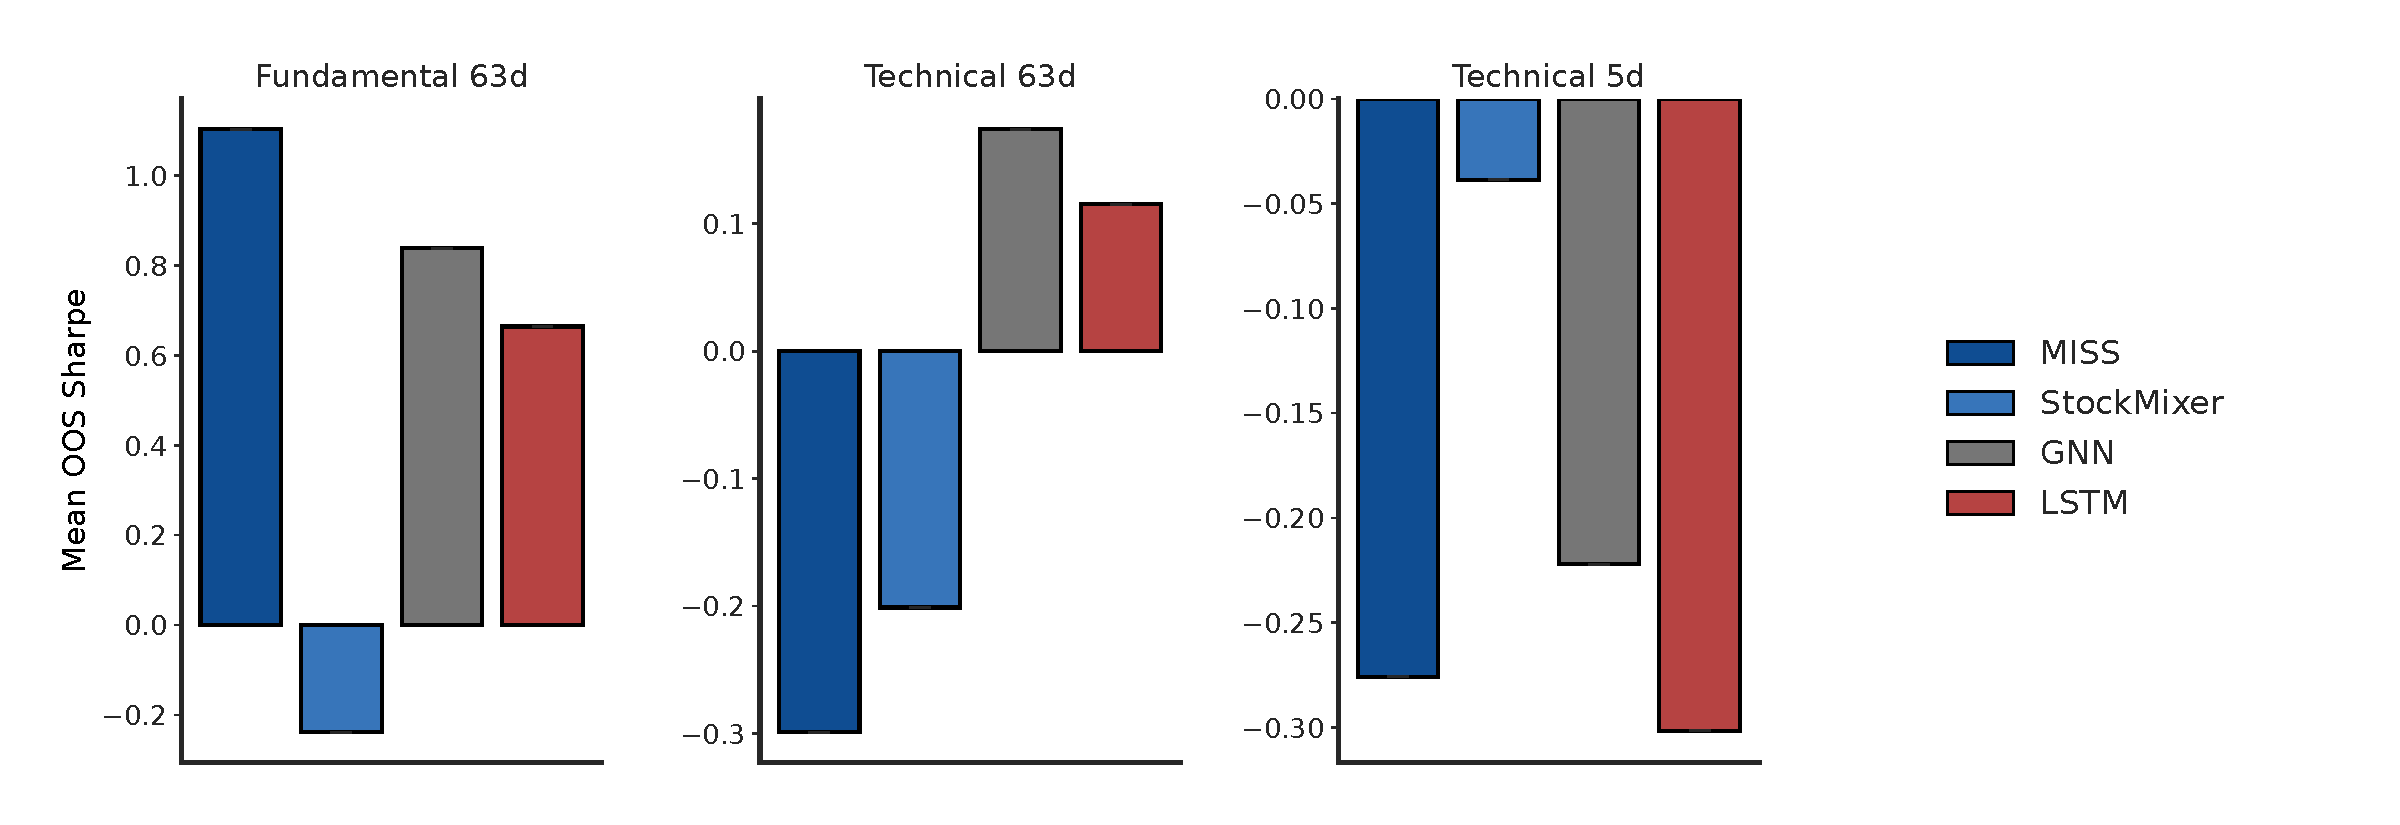
\includegraphics[width=0.92\textwidth]{figures/fig2_arch_sharpe.pdf}
\caption{Mean out-of-sample Sharpe ratio by architecture and information regime (five-year means, net of 15 bps one-way costs). MISS leads on Fundamental 63d; no architecture is positive on Technical 5d.}
\end{figure}
Table 3 gives the portfolio-independent explanation: mean out-of-sample RankIC of the scores. MISS has the strongest sector-demeaned fundamental RankIC (0.039), matching its portfolio rank. StockMixer's fundamental RankIC is negative ($-0.012$), so its last place is a signal failure rather than a backtest artifact. Every technical RankIC lies within $\pm 0.03$ of zero, which is why those portfolios sit at or below zero under any construction.

\begin{table}[t]
\centering\footnotesize
\caption{Mean out-of-sample RankIC (score vs. forward return), 2021--2025, before any portfolio construction.}
\begin{tabular}{l rrrr}
\toprule
Regime & MISS & StkMixer & GNN & LSTM \\
\midrule
Fund. 63d (raw) & 0.027 & $-0.012$ & 0.027 & 0.036 \\
Fund. 63d (dem.) & $\mathbf{0.039}$ & $-0.002$ & 0.033 & 0.033 \\
Tech. 63d (raw) & 0.001 & 0.011 & 0.010 & 0.032 \\
Tech. 5d (raw) & 0.008 & 0.003 & 0.002 & $-0.010$ \\
\bottomrule
\end{tabular}
\end{table}
The fundamental book turns over about 4.7 times NAV per year against roughly 63 for the 5-day book. Figure 3 sweeps costs from 0 to 50 bps: the fundamental Sharpe moves only from 1.136 to 1.028 (return 18.02\% to 16.40\%), while the 5-day technical strategy falls from 0.298 to $-1.558$.

\begin{figure}[t]
\centering
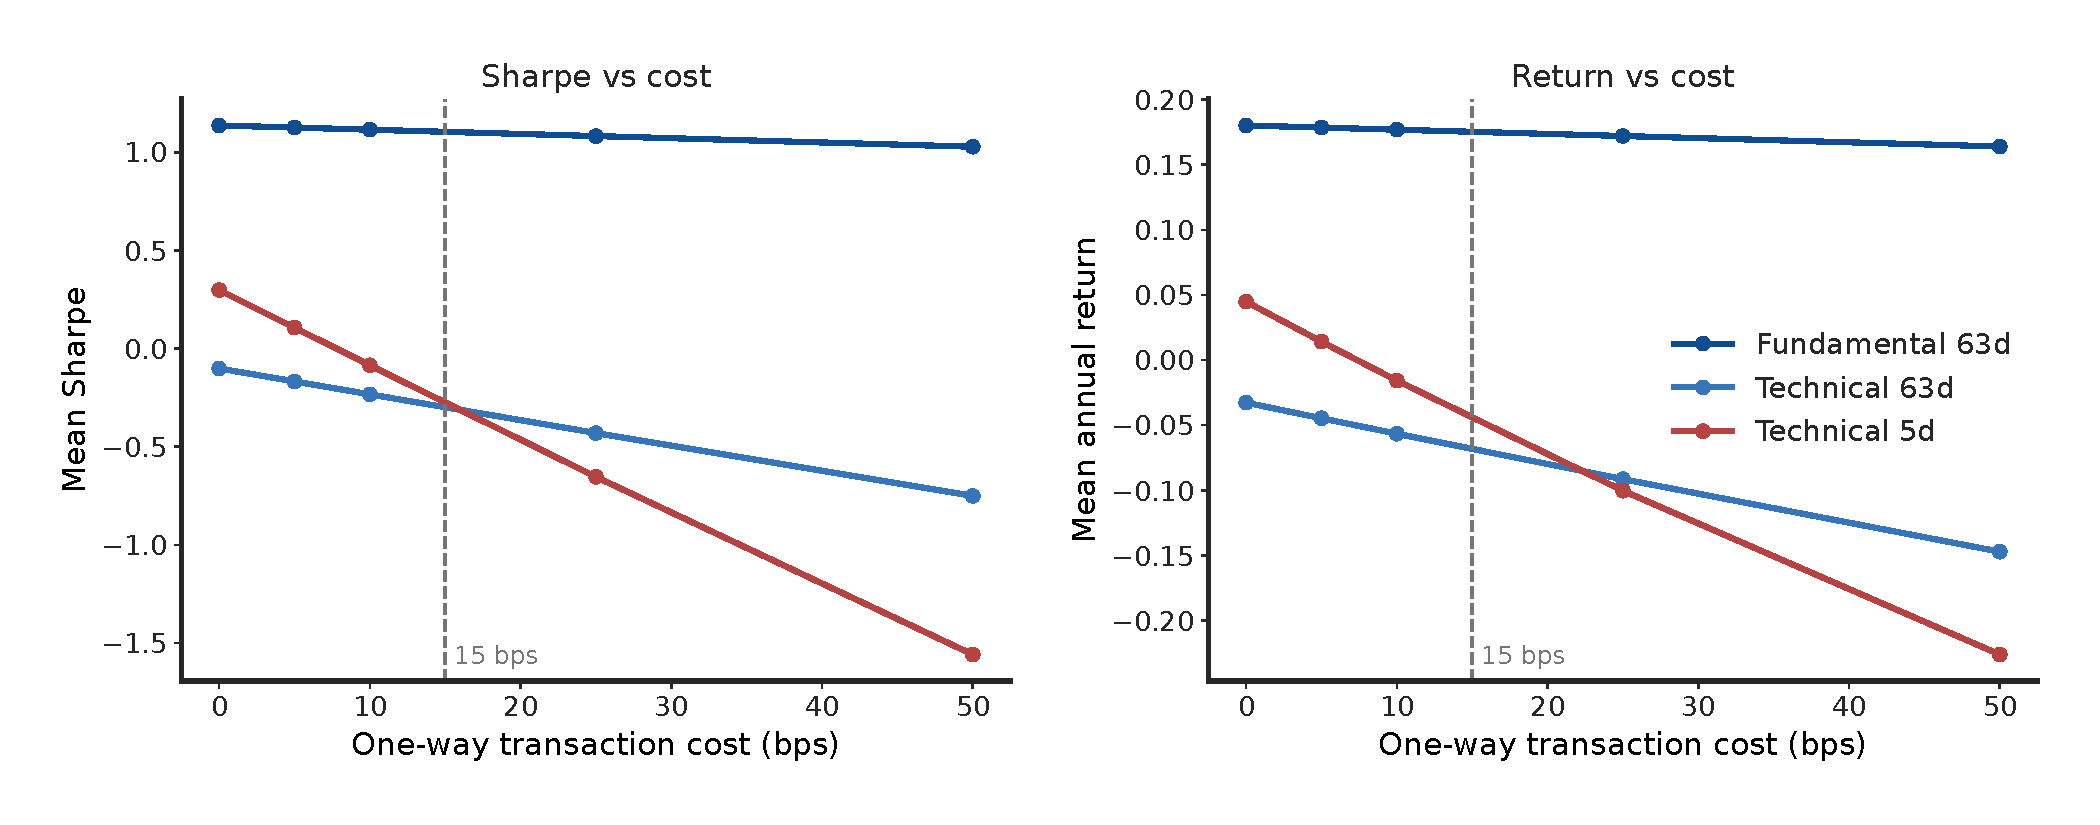
\includegraphics[width=0.92\textwidth]{figures/fig3_cost_sensitivity.pdf}
\caption{Sensitivity of the three MISS strategies to one-way transaction costs, 0--50 bps (five-year means). Dashed line: 15 bps baseline. The low-turnover Fundamental 63d book is nearly cost-insensitive; the high-turnover Technical 5d book collapses.}
\end{figure}
Robustness: the fundamental strategy beats the 5-day technical strategy on annual return in 3 of 5 years (exact one-sided sign test $p = 0.50$) and the 63-day technical strategy in all 5 years ($p = 0.031$). The block bootstrap gives an observed Sharpe difference of 1.520, 95\% interval $[0.215, 2.880]$, $\Pr(\mathrm{diff} > 0) = 0.988$ (Figure 4). The fundamental MISS strategy is the only one of twelve configurations with Deflated Sharpe near 1.0 (benchmark $\mathrm{SR}_0 = 0.828$); the rest are near zero. A vol-matched variant (top-7/bottom-7 at 150\%/150\% gross) returns 31.07\% at Sharpe 0.950 with 27 events per year and 24.7\% realized volatility, showing return and volatility scale with gross exposure while Sharpe barely moves.

\begin{figure}[t]
\centering
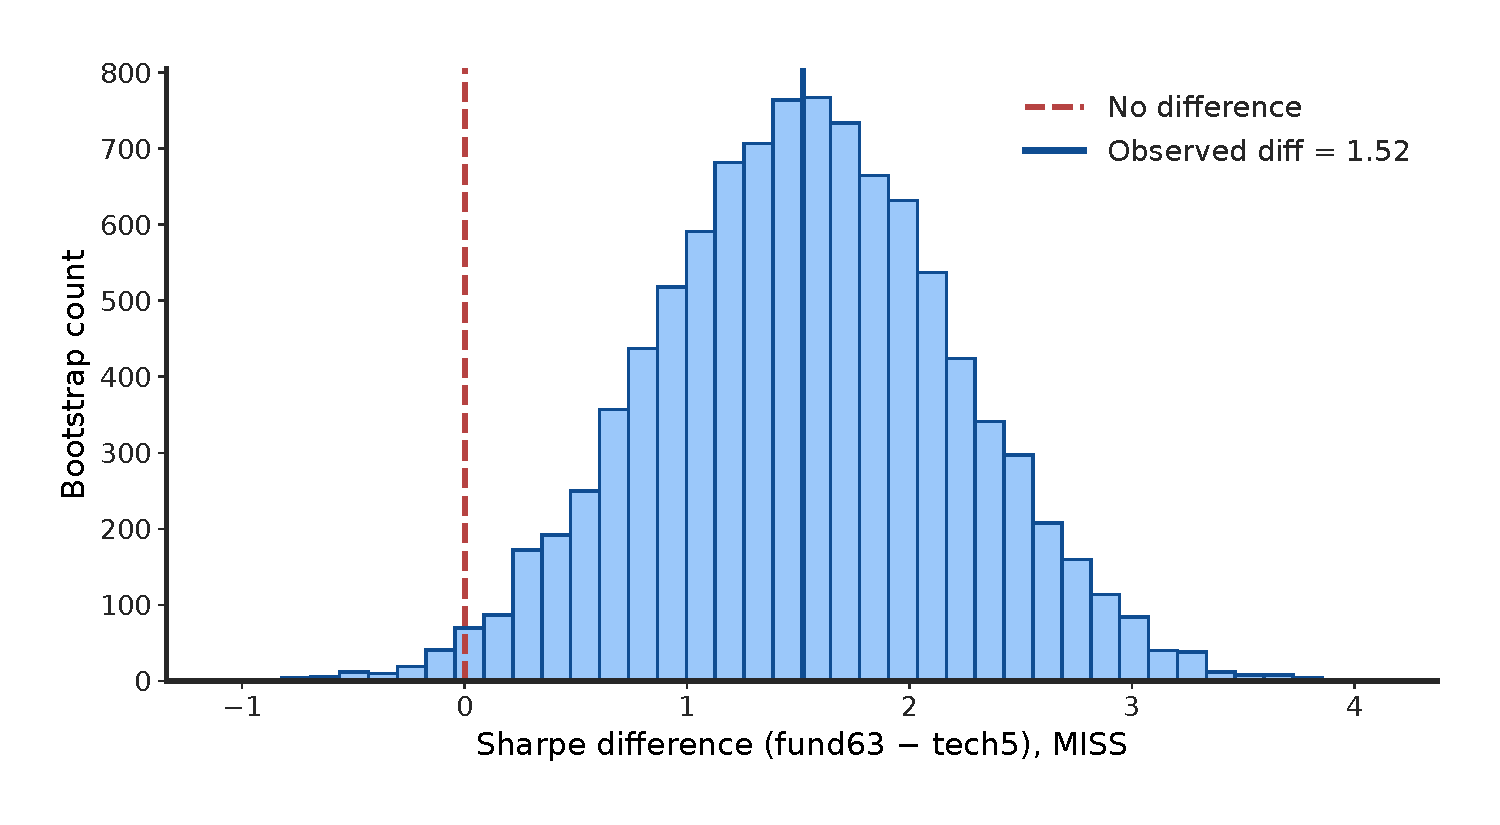
\includegraphics[width=0.92\textwidth]{figures/fig4_bootstrap.pdf}
\caption{Moving-block bootstrap distribution of the Sharpe difference between the fundamental and short-horizon technical MISS strategies (10,000 resamples, 21-day blocks). Observed difference 1.52; $\Pr(\mathrm{diff} > 0) = 0.988$.}
\end{figure}
\section{Discussion}
Across five out-of-sample years, long-horizon fundamental signals beat both technical benchmarks as portfolios, and MISS beat every baseline architecture on fundamentals in both Sharpe (1.104) and signal quality (demeaned RankIC 0.039).

The results support matching the data's frequency, the model's memory, and the portfolio's trading frequency. Mamba's selective memory fits sparse fundamental data: a few observations matter for months. The same architecture shows no edge where the signal is absent, which bounds the claim honestly.

The first objective is met on means and on the 5-of-5 yearly comparison against matched technicals, though the 3-of-5 result against the 5-day strategy is not significant by the sign test alone; the bootstrap is stronger. The second is met for fundamentals; for technicals, no architecture found signal. The third is met: the edge survives 50 bps costs and multiple-testing adjustment.

Future work should widen point-in-time fundamental coverage toward the full 500 names, test longer histories, add factor regressions, and study performance by liquidity and market-cap bucket. Retraining the technical and StockMixer models is the direct route to testing whether their gaps are training artifacts.

Five years cannot cover every regime, and the year path (notably 2021) differs from what a fuller universe might show. Sector neutrality does not remove factor exposures. Costs are modeled flat at 15 bps and vary in practice.

The practical lesson is simple: trade slowly, remember longer, and let the data's own clock set the strategy.

\begin{thebibliography}{16}
\bibitem{fischer2018} T. Fischer, C. Krauss. Deep learning with long short-term memory networks for financial market predictions. European Journal of Operational Research. Vol. 270, pg. 654-669, 2018, https://doi.org/10.1016/j.ejor.2017.11.054.

\bibitem{gkx2020} S. Gu, B. Kelly, D. Xiu. Empirical asset pricing via machine learning. Review of Financial Studies. Vol. 33, pg. 2223-2273, 2020, https://doi.org/10.1093/rfs/hhaa009.

\bibitem{lopez2018} M. Lopez de Prado. \textit{Advances in financial machine learning}. John Wiley \& Sons, 2018.

\bibitem{demiguel2020} V. DeMiguel, A. Martin-Utrera, F. J. Nogales, R. Uppal. A transaction-cost perspective on the multitude of firm characteristics. Review of Financial Studies. Vol. 33, pg. 2180-2222, 2020, https://doi.org/10.1093/rfs/hhz085.

\bibitem{harvey2016} C. R. Harvey, Y. Liu, H. Zhu. ...and the cross-section of expected returns. Review of Financial Studies. Vol. 29, pg. 5-68, 2016, https://doi.org/10.1093/rfs/hhv059.

\bibitem{gu2023} A. Gu, T. Dao. Mamba: linear-time sequence modeling with selective state spaces. arXiv:2312.00752, 2023.

\bibitem{shiller1981} R. J. Shiller. Do stock prices move too much to be justified by subsequent dividends? American Economic Review. Vol. 71, pg. 421-436, 1981.

\bibitem{bailey2014} D. H. Bailey, M. Lopez de Prado. The deflated Sharpe ratio: correcting for selection bias, backtest overfitting, and non-normality. Journal of Portfolio Management. Vol. 40, pg. 94-107, 2014.

\bibitem{yahoo2026} Yahoo Finance. Historical market data and price history. 2026, https://finance.yahoo.com.

\bibitem{sec2025} U.S. Securities and Exchange Commission. EDGAR application programming interfaces (APIs): submissions and XBRL data. SEC.gov, 2025, https://www.sec.gov/edgar/sec-api-documentation.

\bibitem{hochreiter1997} S. Hochreiter, J. Schmidhuber. Long short-term memory. Neural Computation. Vol. 9, pg. 1735-1780, 1997, https://doi.org/10.1162/neco.1997.9.8.1735.

\bibitem{rumelhart1986} D. E. Rumelhart, G. E. Hinton, R. J. Williams. Learning representations by back-propagating errors. Nature. Vol. 323, pg. 533-536, 1986.

\bibitem{fan2024} J. Fan, Y. Shen. StockMixer: a simple yet strong MLP-based architecture for stock price forecasting. Proceedings of AAAI. Vol. 38, pg. 8389-8397, 2024, https://doi.org/10.1609/aaai.v38i8.28681.

\bibitem{feng2019} F. Feng, X. He, X. Wang, C. Luo, Y. Liu, T.-S. Chua. Temporal relational ranking for stock prediction. ACM Transactions on Information Systems. Vol. 37, 2019, https://doi.org/10.1145/3309547.

\bibitem{qian2024} H. Qian, et al. MDGNN: multi-relational dynamic graph neural network for comprehensive and dynamic stock investment prediction. Proceedings of AAAI. Vol. 38, 2024, https://doi.org/10.1609/aaai.v38i13.29381.

\bibitem{vaswani2017} A. Vaswani, et al. Attention is all you need. Advances in Neural Information Processing Systems. Vol. 30, 2017.

\end{thebibliography}

\end{document}
